%!TEX root = thesis.tex
% !TEX spellcheck = en-US
\chapter[Background]{Background}

\section{Energy efficiency} \label{energymeasurement}
Computers consume energy.
Achieving low energy consumption is an area of great interest, both in super computers where power is expensive and in consumer hardware where low power mean longer battery life.
The energy consumption of a system depend both on hardware and software.
The hardware of the system will typically run within a narrow range of voltages, and the components of the system have some current drag when they are working.
The programmer can not affect how large these values are.
What can be done however, is to ensure that the software does not consume energy unnecessary.
The some of the components in the system that are not used can be turned off.
Some of the features of a processor may also cause it to consume more power.
An example is NEON vector instructions, which have been shown to increase the power usage of the system by up to 20\%\cite{TrondIngeLillesand} when used.
Turning off components or features does save power, but there will often be a performance loss.
When energy efficiency is a goal, there is always questions about how much power can be saved before the execution time is extended so much that there is a total loss in power consumed.
Because of this, it is interesting to analyze programs with regard to energy consumption.

\subsubsection{Energy measurement}
There as mentioned, the interesting power properties of a system is voltage and current.
In systems featuring sensors for such data, the data can be gathered while executing a program.
By analyzing the data it is possible to optimize the program for energy efficiency.

The power of the system is the product of the voltage and current.
This is interesting to observe in applications that run when the system is standing by.
When execution time doesn't matter, the energy consumed per time is what matter.

Often the system is executing a program for a duration, and as soon as it is done the system can be shut down.
In such cases it is interesting to measure how much energy the system consumed during execution.
The product of the systems power and the problems execution time, is the total amount of energy consumed.

There are many cases where a balance between energy efficiency and the performance trade off is interesting.
This is when the energy delay product of the system become interesting.
This is valid both for scientific experiments and programs executed on regular systems.
In research experiments the goal may be to obtain energy efficiency or performance.
In either case, it is sensible to remember that the actual goal will normally be a balance between the two.
On regular systems in real life applications, both energy and performance matter.
Users does not want to wait longer than necessary for the system to complete its task.
Neither do they want the system to run out of battery or the power bill to grow too big.
The energy delay product of a system is calculated by multiplying the execution time of the application with its energy.

\section{NEON}
NEON is a general-purpose single input multiple data (SIMD) technology implemented in the ARM Cortex A series of processors.
It is able to run SIMD instructions on 128bit registers.
By utilizing the NEON unit of the ARM processors, it is possible to achieve parallelism in each separate core.
This will often open for great performance boost on problems like the ones explored in this paper.
Each register may be filled with single precision floating point numbers ranging from 8 to 64 bit each.
In future generations of the ARM ISA there will be support for other data types as well.
Different implementations of NEON exist in the Cortex A cores, and while the even the simple implementations in smaller cores like the A7 can give great performance boost, the implementations present in the newest cores are performing even better.
The A15 offer two NEON units, and the instruction pipeline to start the cores are shorter than in simpler implementations.

\section{Task based programming}
Task based programming allow a programmer to work with parallel programs, with an abstraction from the parallelization itself.
When programming with this model, the program can be split into tasks which can run in parallel.
When the program run, it will run a task manager as part of the program.
This task manager can dynamically assign tasks to the processors, and the programmer does not have to handle all the time consuming tasks related to manual parallelization.
As long as the programmer correctly handle dependencies in the parallelized code, it will be possible to write this kind of code as if it was serial.

The task based programming model also allow simpler development of portable programs.
When the program is running tasks on available CPUs, it is not a problem to allow it to run on larger or smaller numbers of processors, and even clusters can support the program.
This model even allow the tasks to run on different types of processors in a heterogeneous environment.

\section[OmpSs]{OpenMP Super scalar}
OpenMP Super scalar (OmpSs) is a extension of the OpenMP API to integrate features from the StarSs programming model.
It is currently under development at the Barcelona Supercomputing Center.
The goal of OmpSs is to extend the programming model to support a wide range of processors.
The OmpSs programming model will run on a wide variety of different systems, such as traditional personal computers, clusters, shared memory systems and heterogeneous processors.
While the software is not yet completed or fully tested, there have been several reports exploring it's potential.
The results have proven OmpSs as an efficient solution on both clusters and heterogeneous systems utilizing OpenCL and CUDA.


\section{Heterogeneous multi-processor}
Heterogeneous multi-processor systems have multiple different processors, opposed to traditional multi-processor systems.
A typical modern processor have several processors, and a program can run effectively by having threads running parts of thesis work on each of them.
This work is often of such a nature that it can run better on a different processor.
Sometimes it can run just as well on multiple simple processor, while using less die space and energy.
In other instances, an advanced processor with some special capabilities, like vector instructions, can be more efficient.

  This kind of processors have a potential to help us overcome the challenges that are emerging in processor development.
    Unfortunately they also introduce several new challenges.

\section{Experiment platforms}

\subsection{Arndale Board} \label{ArendaleBoard}
\begin{figure}[ht!]
  \centering
  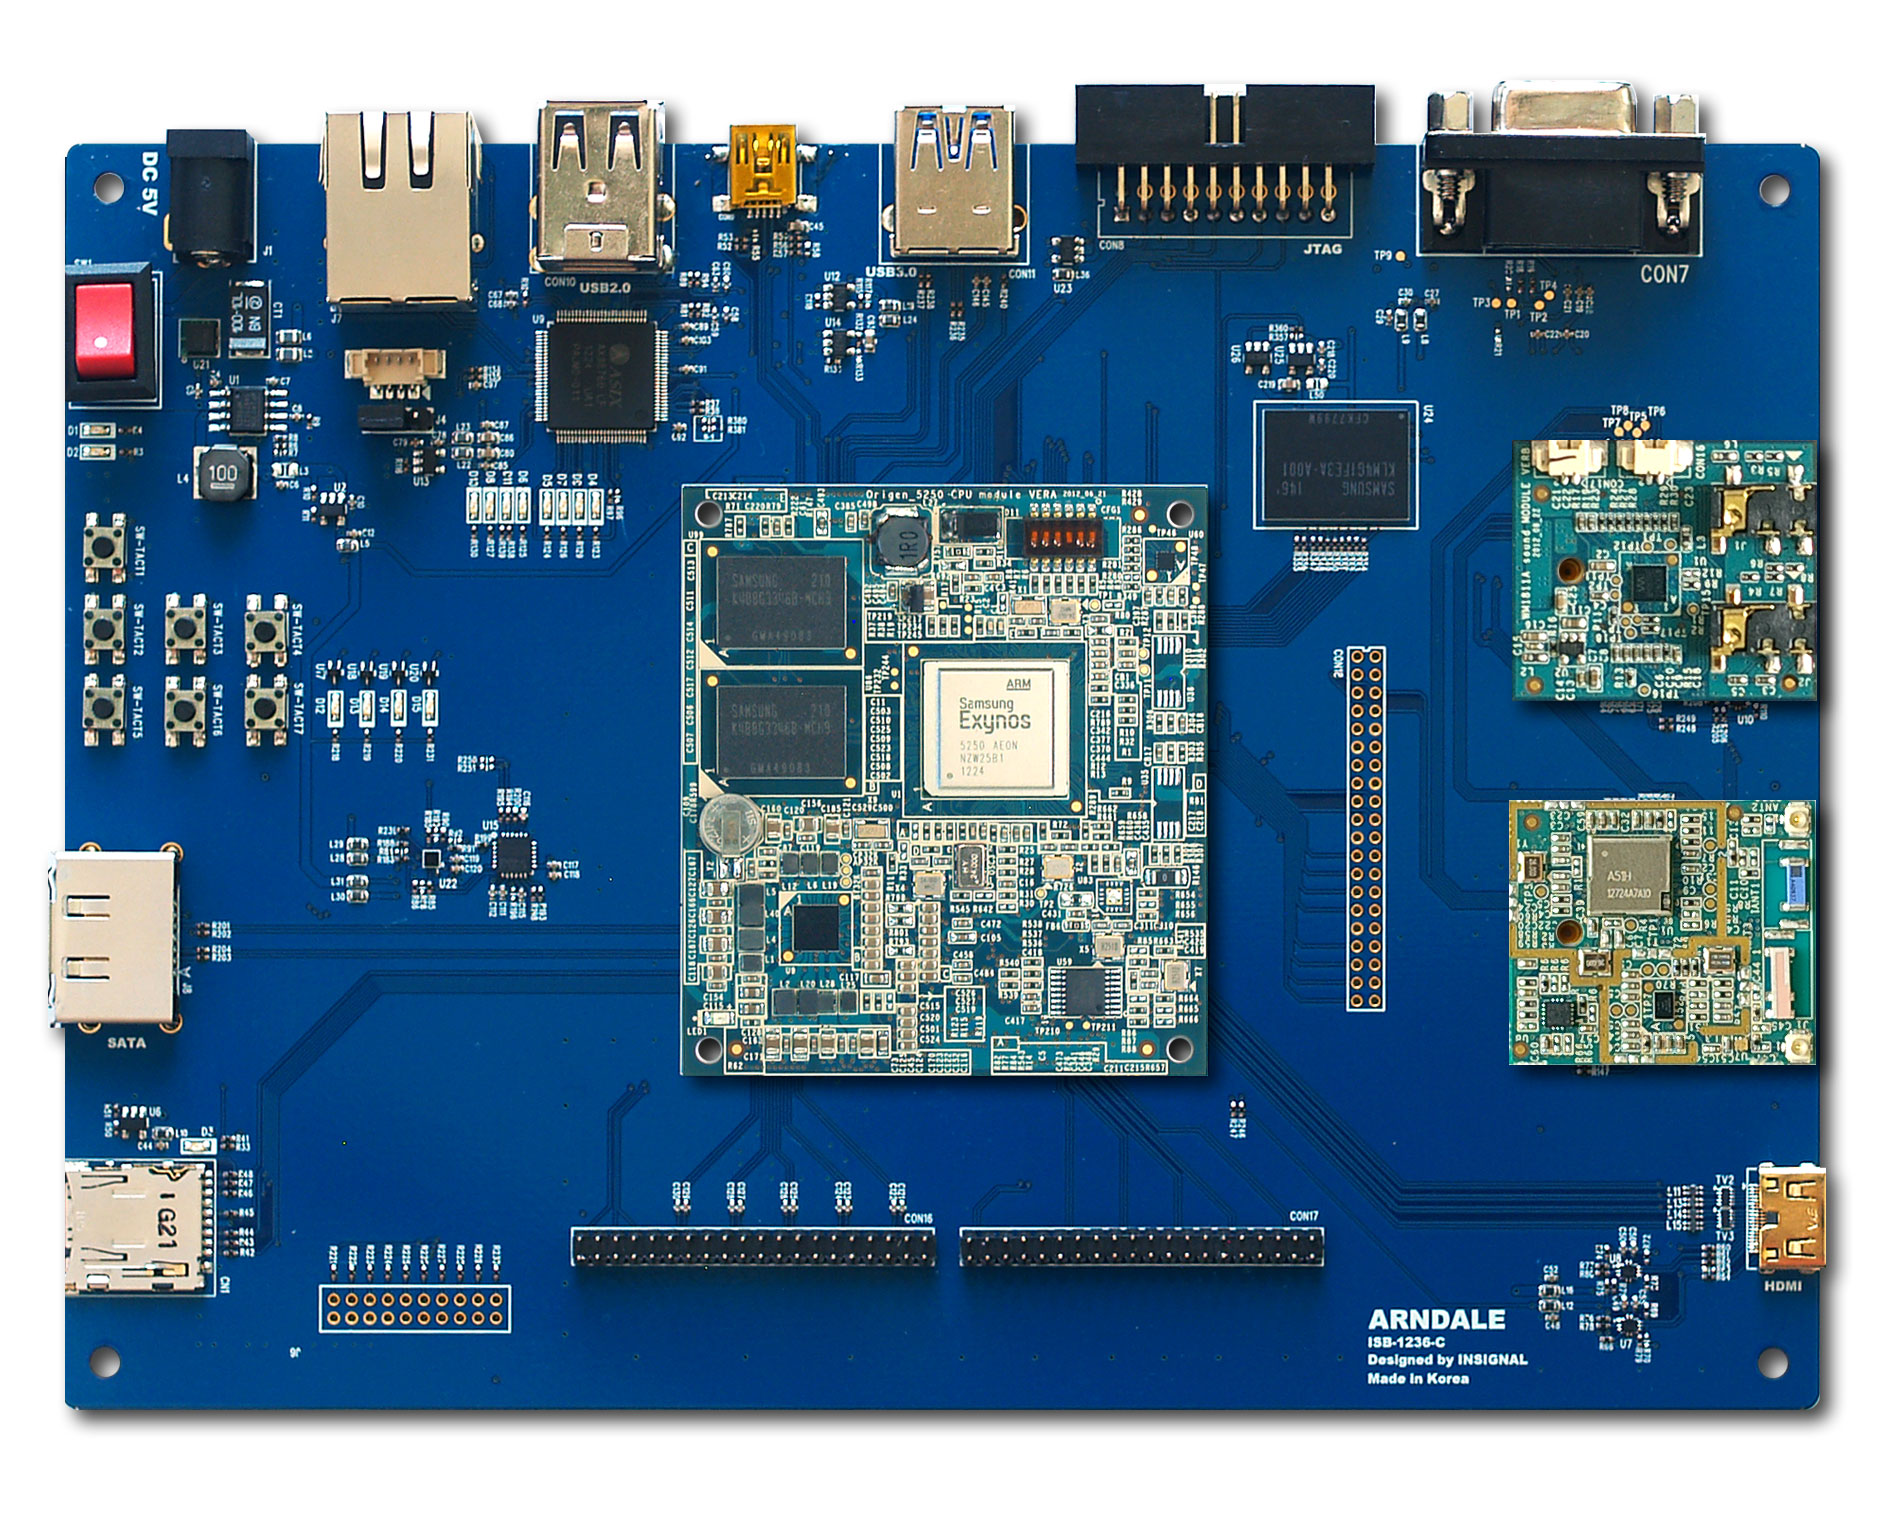
\includegraphics[width=90mm]{fig/Arendale.jpg}
  \caption{Arndale Duo \label{overflow}}
\end{figure}
The Arndale Duo is a computing system mounted on a single board.
It is fitted with an Exynos 5250 SoC, which contain a dual core Arm Cortex-A15 , as well as an ARM Mali T-604 GPU.
This computer offer a range of supported Linux distributions, as well as the OmpSs programming model.
The computer was used in the 2014 master thesis "Acceleration with OmpSs and Neon/OpenCL on ARM Processor" by Trond Inge Lillesand.
The thesis lay a lot of the ground for this pilot project and planned master thesis.

\subsection{ODROID-XU3} \label{OdroidXU3}
\begin{figure}[ht!]
  \centering
  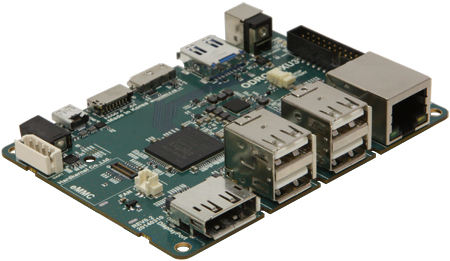
\includegraphics[width=90mm]{fig/ODROID.jpg}
  \caption{ODROID-XU3 \label{overflow}}
\end{figure}
The ODROID-XU3 is a new single-board computing system, offering interesting properties for these experiments.
The system has an Exynos 5422 heterogeneous Soc.
Exynos 5422 has a quad core ARM Cortex-A15 CPU and a ARM Mali T-628 GPU, but also a smaller quad core ARM Cortex-A7 processor.
These 3 different processing units can be used simultaneously to solve problems.
In this paper, and the planned master thesis following it, the potency of this kind of heterogeneous processor will be explored.

\subsubsection{Power monitoring}
The ODROID-XU3 comes with integrated power monitoring tools.
Implemented in hardware, it have got 4 current sensors sitting on the power pins of the Exynos SoC.
The energy monitors are indicated in figure \ref{overview-odroid}.
These monitor the current going through the large CPU cores, the small CPU cores, memory and GPU respectively.
In addition to the current sensors, the power management for the SoC is also available to the programmer, making supply voltage to the components known.
By using the voltage and current, the power consumption is known.
As a whole, the system offer frequency, voltage, current, temperature and power readings in real time.
These fine energy and performance metrics make the system highly suitable for developers.
They are able to run their programs, collect energy profiling data and optimize their software based on the result.

\begin{figure}[ht!]
  \centering
  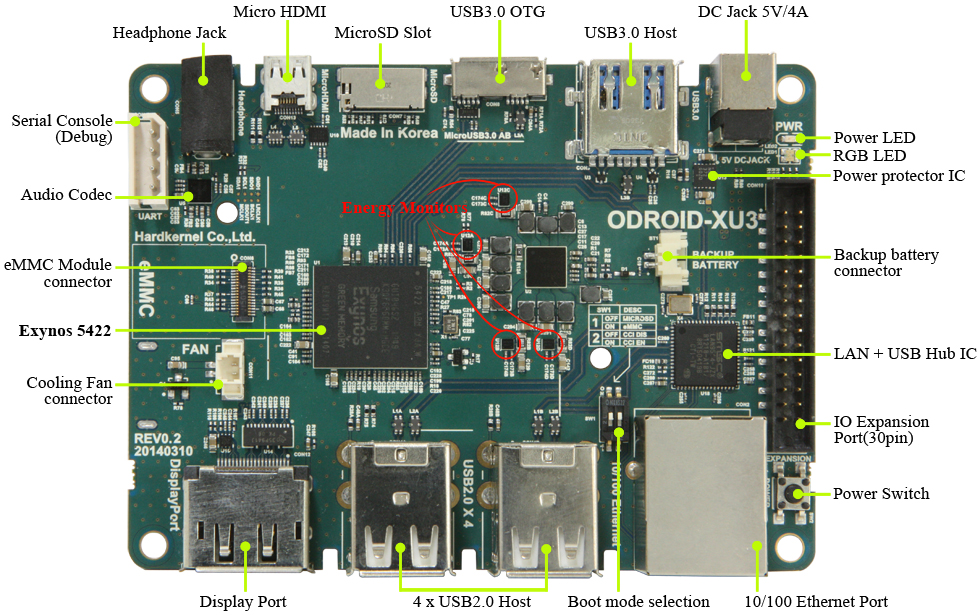
\includegraphics[width=130mm]{fig/overview-odroid.jpg}
  \caption{ODROID-XU3 annotated (hardkernel.com\cite{hardkernel01})\label{overview-odroid}}
\end{figure}

\subsubsection{Performance}

The ODROID-XU3 comes with the ARM Cortex-A15 limited to 2GHz and the ARM Cortex-A7 limited to 1.4G Hz.
There is 2GB of memory available running at 800 MHz, and the ARM Mali T-628 GPU run at 600 MHz.
This performance place it at the higher end of SoCs, but not quite in the top, as it is beaten by systems like TODO A reference system here).
The ODROID-XU3 feature the new eMMC 5.0 standard for storage.
The performance of this standard outperform both older eMMC standards, as well as memory card readers, which other similar systems may contain.
The ODROID-XU3 can achieve a read/write performance of 198/74 MB/s\cite{hardkernel01}, which a lot better than older systems like the Arndale Duo.

In addition to the eight processor cores, the system also feature a ARM Mali T-628.
The Mali T-628 function both as a regular GPU, as well as a GPGPU.
It support both openGL and DirectX, and is able to produce graphics for all but the most demanding gaming and simulation purposes.
In addition to this it is able to run computations with Open CL.
This mean that problems with parallel parts, can be solved efficiently utilizing the GPU.

\subsection{ARM Cortex-A15}
\begin{table}[H]
  \begin{tabular}{ll}
    Performance       & 1.0 GHz to 2.5GHz  \\
    L1 Cache          & 64KB \\
    L2 Cache          & 4 MB \\
    L3 Cache          & None in core, may be implemented shared in multi core system. \\Architecture      & ARMv7-A            \\
    Architecture      & ARMv7-A            \\
                      & TrustZone® security technology \\
                      & NEON™ Advanced SIMD \\
                      & DSP \& SIMD extensions \\
                      & VFPv4 Floating point \\
                      & Hardware vitalization support \\
                      & Integer Divide \\
                      & Fused MAC \\
                      & Hypervisor debug instructions \\
    Memory management & 40-bit ARMv7 Memory Management Unit
  \end{tabular}
\end{table}
\subsection{ARM Cortex-A7}
The ARM Cortex-A7 is designed to be a low power alternative to the ARM Cortex-A15 and ARM Cortex-A17, with the same supported ISA and features.
This enable the ARM Cortex to be paired with it's larger relatives in a ARM big.LITTLE configuration.
\begin{table}[H]
  \begin{tabular}{ll}
    Performance       & 1.2 GHz to 1.6GHz  \\
    L1 Cache          & 8-64KB \\
    L2 Cache          & up to 1 MB \\
    L3 Cache          & None in core, may be implemented shared in multi core system. \\
    Architecture      & ARMv7-A            \\
    Supported features& ARM Thumb-2 \\
                      & TrustZone® security technology \\
                      & NEON™ Advanced SIMD \\
                      & DSP \& SIMD extensions \\
                      & VFPv4 Floating point \\
                      & Hardware vitalization support \\
                      & Integer Divide \\
                      & Fused MAC \\
                      & Hypervisor debug instructions \\
    Memory management & 40-bit ARMv7 Memory Management Unit
  \end{tabular}
\end{table}
\subsection{ARM Mali T604}
\begin{table}[H]
  \begin{tabular}{ll}
    Performance       & 533 MHz\\
                      & 17 GFLOPS  \\
    Multi core support & 1-4 cores  \\
    API Support       & OpenGL 1.1, 2.0, 3.0 and 3.1  \\
                      & OpenCL 1.1  \\
                      & DirectX 11  \\
                      & RenderScript \\
    Anti-Aliasing     & 4xFSAA with minimal performance drop  \\
                      & 16xFSAA  \\
    Cache             & 32-256KB L2 cache
  \end{tabular}
\end{table}
\subsection{ARM Mali T628}
\begin{table}[H]
  \begin{tabular}{ll}
    Performance       & 533/695 MHz \\
                      & 17/23.7 GFLOPS \\
    Multi core support & 1-8 cores  \\
    API Support       & OpenGL 1.1, 2.0, 3.0 and 3.1  \\
                      & OpenCL 1.1  \\
                      & DirectX 11  \\
                      & RenderScript \\
    Anti-Aliasing     & 4xFSAA with minimal performance drop  \\
                      & 16xFSAA  \\
    Cache             & 32-256KB L2 cache
  \end{tabular}
\end{table}

\section{Algorithms}
Here I will write about the algorithms used in the experiments.

